% Generated by pysimcount.pfboundratio -- do not edit; regenerate instead.
% figure: bound-ratio-suzuki2 -- Suzuki S2: Trotter number from each bound / measured r, against n
% metric=r_ratio gatebase=cz; geometric mean over seeds [1, 2, 3, 4, 5, 6, 7, 8, 9, 10], bars min-max; r_method=measured (denominator); bounds: Analytic bound, Minimised bound, Commutator bound (2018), Commutator bound (2021), Empirical fit (2018)
% sizes: np-main n = [4, 5, 6, 7, 8, 10]; np-main-n9 n = [9]; np-main-n11 n = [11]
% run set np-main-n9 made from uncommitted code (git_dirty), accepted: run at e42ff29 with the only modified tracked file pysimcount/pfseeds.py (an aggregation module the run does not import); checked with git diff --stat e42ff29 -- pysimcount/ on 2026-11-08
% run set np-main-n11 made from uncommitted code (git_dirty), accepted: run at e42ff29 with the only modified tracked file pysimcount/pfseeds.py (an aggregation module the run does not import); checked with git diff --stat e42ff29 -- pysimcount/ on 2026-11-08
% formulas: Suzuki S2
% figure made at git_commit=e5d9ee696f892e28aced765585653760f8a427c4 git_dirty=False
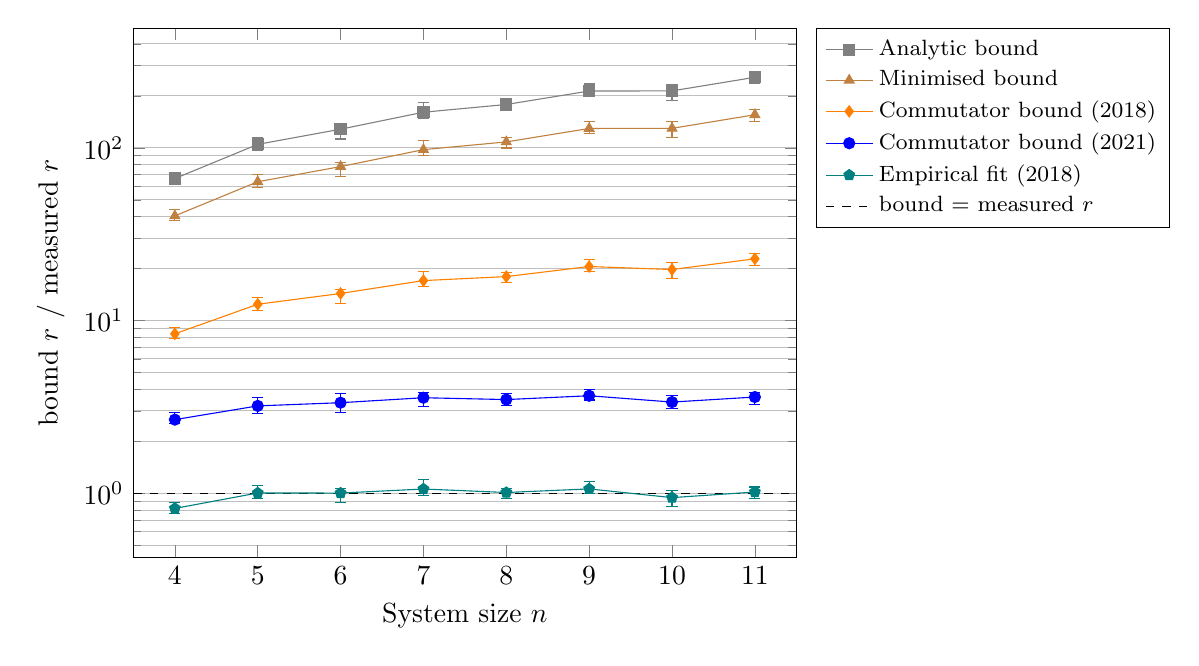
\begin{tikzpicture}
  \begin{semilogyaxis}[
    width=10cm, height=8.3cm,
    xlabel={System size $n$}, ylabel={bound $r$ / measured $r$},
    xmin=3.5, xmax=11.5,
    xtick={4,5,6,7,8,9,10,11},
    ymajorgrids=true, yminorgrids=true,
    legend pos=outer north east, legend cell align=left,
    legend style={font=\footnotesize},
  ]
    \addplot[dashed, black, domain=3.5:11.5, samples=2, forget plot] {1};
    \addplot[solid, gray, mark=square*, mark size=2pt, error bars/.cd, y dir=both, y explicit] coordinates {
      (4,66.4196) -= (0,4.05627) += (0,5.75254)
      (5,104.724) -= (0,7.8636) += (0,10.4861)
      (6,128.209) -= (0,15.7301) += (0,7.38767)
      (7,160.735) -= (0,12.4965) += (0,21.3569)
      (8,178.191) -= (0,13.9277) += (0,10.2105)
      (9,213.209) -= (0,12.6699) += (0,20.8951)
      (10,213.59) -= (0,24.9148) += (0,20.3102)
      (11,256.02) -= (0,20.8533) += (0,17.6194)
    };
    \addlegendentry{Analytic bound}
    \addplot[solid, brown, mark=triangle*, mark size=2pt, error bars/.cd, y dir=both, y explicit] coordinates {
      (4,40.3832) -= (0,2.46622) += (0,3.49755)
      (5,63.6411) -= (0,4.77875) += (0,6.37244)
      (6,77.888) -= (0,9.55615) += (0,4.48808)
      (7,97.6255) -= (0,7.58996) += (0,12.9715)
      (8,108.21) -= (0,8.4578) += (0,6.20048)
      (9,129.457) -= (0,7.69295) += (0,12.6872)
      (10,129.674) -= (0,15.1262) += (0,12.3307)
      (11,155.421) -= (0,12.6593) += (0,10.6961)
    };
    \addlegendentry{Minimised bound}
    \addplot[solid, orange, mark=diamond*, mark size=2pt, error bars/.cd, y dir=both, y explicit] coordinates {
      (4,8.38473) -= (0,0.512059) += (0,0.726193)
      (5,12.4355) -= (0,0.933768) += (0,1.24518)
      (6,14.3536) -= (0,1.76105) += (0,0.827084)
      (7,17.0447) -= (0,1.32515) += (0,2.26474)
      (8,17.981) -= (0,1.40542) += (0,1.03032)
      (9,20.5594) -= (0,1.22173) += (0,2.01488)
      (10,19.7554) -= (0,2.30442) += (0,1.87854)
      (11,22.787) -= (0,1.85605) += (0,1.56822)
    };
    \addlegendentry{Commutator bound (2018)}
    \addplot[solid, blue, mark=oplus*, mark size=2pt, error bars/.cd, y dir=both, y explicit] coordinates {
      (4,2.67147) -= (0,0.131241) += (0,0.280516)
      (5,3.2085) -= (0,0.318852) += (0,0.376055)
      (6,3.34785) -= (0,0.398309) += (0,0.438961)
      (7,3.57745) -= (0,0.39831) += (0,0.247957)
      (8,3.49092) -= (0,0.260114) += (0,0.289739)
      (9,3.6735) -= (0,0.203411) += (0,0.301984)
      (10,3.37633) -= (0,0.294608) += (0,0.289196)
      (11,3.61092) -= (0,0.343992) += (0,0.203751)
    };
    \addlegendentry{Commutator bound (2021)}
    \addplot[solid, teal, mark=pentagon*, mark size=2pt, error bars/.cd, y dir=both, y explicit] coordinates {
      (4,0.818209) -= (0,0.0499683) += (0,0.0708642)
      (5,1.00492) -= (0,0.0754588) += (0,0.100624)
      (6,1.0039) -= (0,0.12317) += (0,0.0578472)
      (7,1.05953) -= (0,0.082374) += (0,0.14078)
      (8,1.01172) -= (0,0.0790773) += (0,0.0579722)
      (9,1.06103) -= (0,0.0630515) += (0,0.103984)
      (10,0.944839) -= (0,0.110213) += (0,0.0898447)
      (11,1.01807) -= (0,0.0829241) += (0,0.0700644)
    };
    \addlegendentry{Empirical fit (2018)}
    \addlegendimage{dashed, black}
    \addlegendentry{bound $=$ measured $r$}
  \end{semilogyaxis}
\end{tikzpicture}
